\documentclass{beamer}
\usetheme{metropolis}           % Use metropolis theme
\usepackage[utf8]{inputenc}
\usepackage{soul}
\usepackage{float}
\usepackage{caption}
\usepackage{subcaption}
\usepackage[brazil]{babel} % Idioma do documento
\usepackage[style = abnt, backend = biber]{biblatex}
\addbibresource{refs.bib}
\title{Emergência de Distribuições de Preferência no caso Unidimensional: uma
  abordagem computacional}
\date{}
\author{Marcelo Veloso Maciel}
\institute{}
\begin{document}
\maketitle



% ----------------- NOVO SLIDE --------------------------------
\begin{frame}{Sumário}
\tableofcontents
\end{frame}



\section{Introdução}
\begin{frame}{Objetivo}
  Propor e analisar um modelo generativo de Opinião Pública
\end{frame}


\begin{frame}{Justificativa}
  \begin{itemize}
  \item Normativa
  \item Positiva
  \end{itemize}
\end{frame}

\begin{frame}{Escopo}
  \begin{itemize}
  \item Sistema Alvo \(\rightarrow\) Opiniões Públicas Nacionais
  \item Microfundamentos da Opinião Pública = Opinião Idiossincrática +
    Influência Social (Pares e \st{Mídia} )
  \end{itemize}
  
\end{frame}

\section{Fundamentação Teórica}
\begin{frame}{Literaturas}

Critérios de Fidelidade \cite{weisberg2012simulation}:
\begin{itemize}
\item Estrutura;
\item \textit{Output}.
\end{itemize}
  
Base para a construção do modelo:

\begin{itemize}
\item Teoria Política Formal
\item Dinâmicas de Opinião
\item \textcolor{gray!70}{Opinião Pública}
\end{itemize}
\end{frame}

\begin{frame}{Teoria Política Formal}

  \begin{itemize}
  \item Definição: Modelagem Formal de Política;
  \item Principal subconjunto: Teoria da Escolha Racional;
  \item Modelo do ator racional: Preferências Transitivas + Atualização
    Bayesiana.
  \end{itemize}

\end{frame}


\begin{frame}{Teoria Espacial e Eleições: Microfundamentos I}
  \begin{itemize}
  \item Teoria Política Espacial : analogia espacial;
  \item Comitês x Eleições de Larga Escala;
  \item Atitudes e  Ideologia.
  \end{itemize}
\end{frame}

\begin{frame}{Teoria Espacial e Eleições: Macrofundamentos I }
  \begin{itemize}
\item \textcite{druckman2012public} aponta dois achados canônicos da Opinião
  Pública:
  \begin{itemize}
  \item Instabilidade Micro;
  \item Estabilidade Macro.
  \end{itemize}
  \end{itemize}
  
\end{frame}


\begin{frame}{Teoria Espacial e Eleições: Macrofundamentos I }
  \begin{figure}[H]
    \centering
    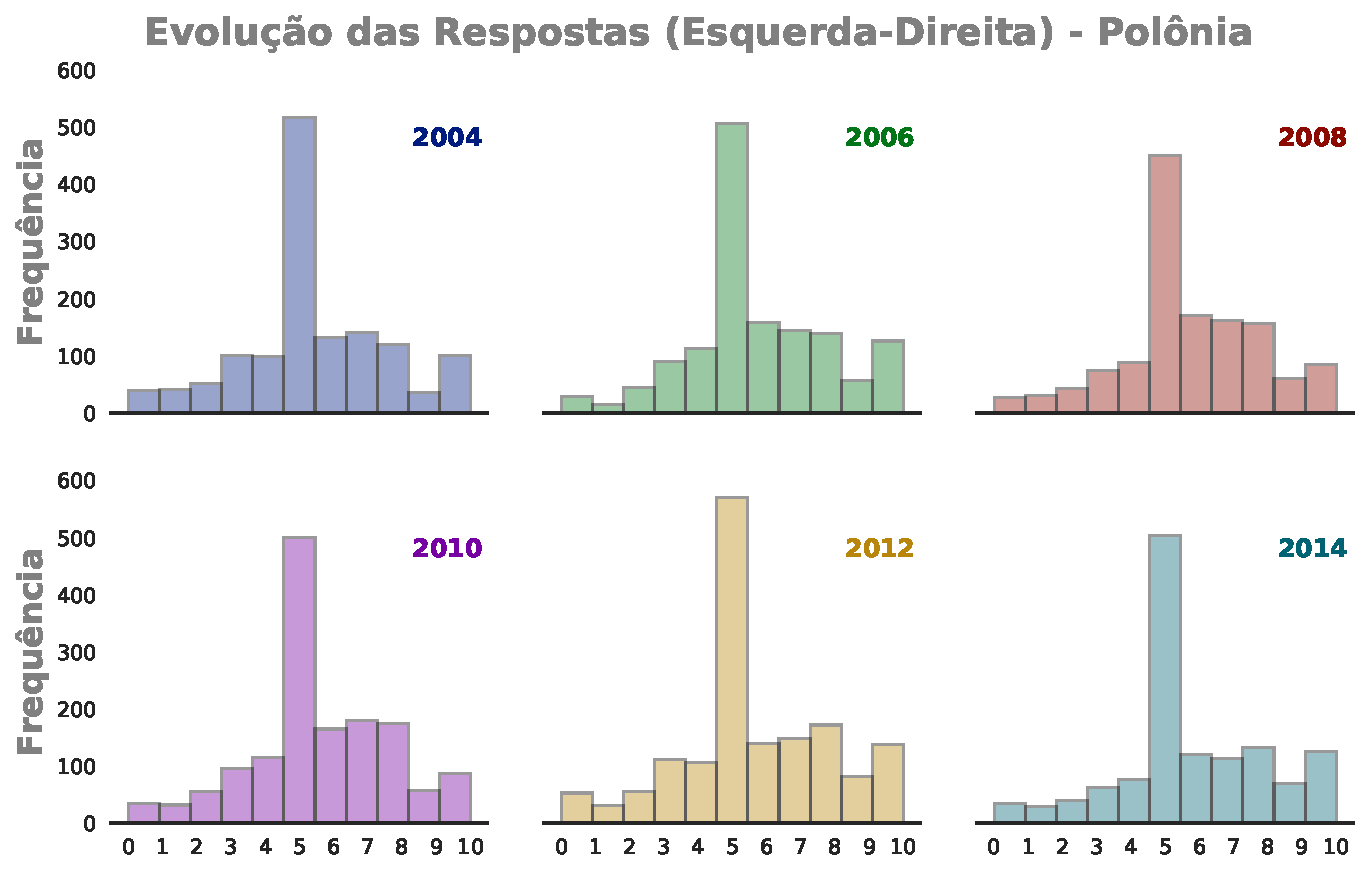
\includegraphics[scale = 0.4]{ims/ess_Pol_plots.pdf}
    \caption{Estabilidade Ideológica}
    \label{fig1}
  \end{figure}
\end{frame}


\begin{frame}{Teoria Espacial e Eleições: Macrofundamentos II}

  \begin{itemize}

  \item Partidos e Relevo Eleitoral
 \item \textcite{flache2017} aponta os seguintes fatos estilizados sobre
   distribuições de opinião pública no ESS:
   
    \begin{itemize}

    \item  há um pico central dominante;
    \item há uma tendência para a existência de \textit{clusters} não centrais;
    \item há uma tendência a picos nos extremos.
      
    \end{itemize}
    
  \end{itemize}
  
\end{frame}

\begin{frame}{Teoria Espacial e Eleições: Macrofundamentos II}  
  \begin{figure}[H]
      \centering 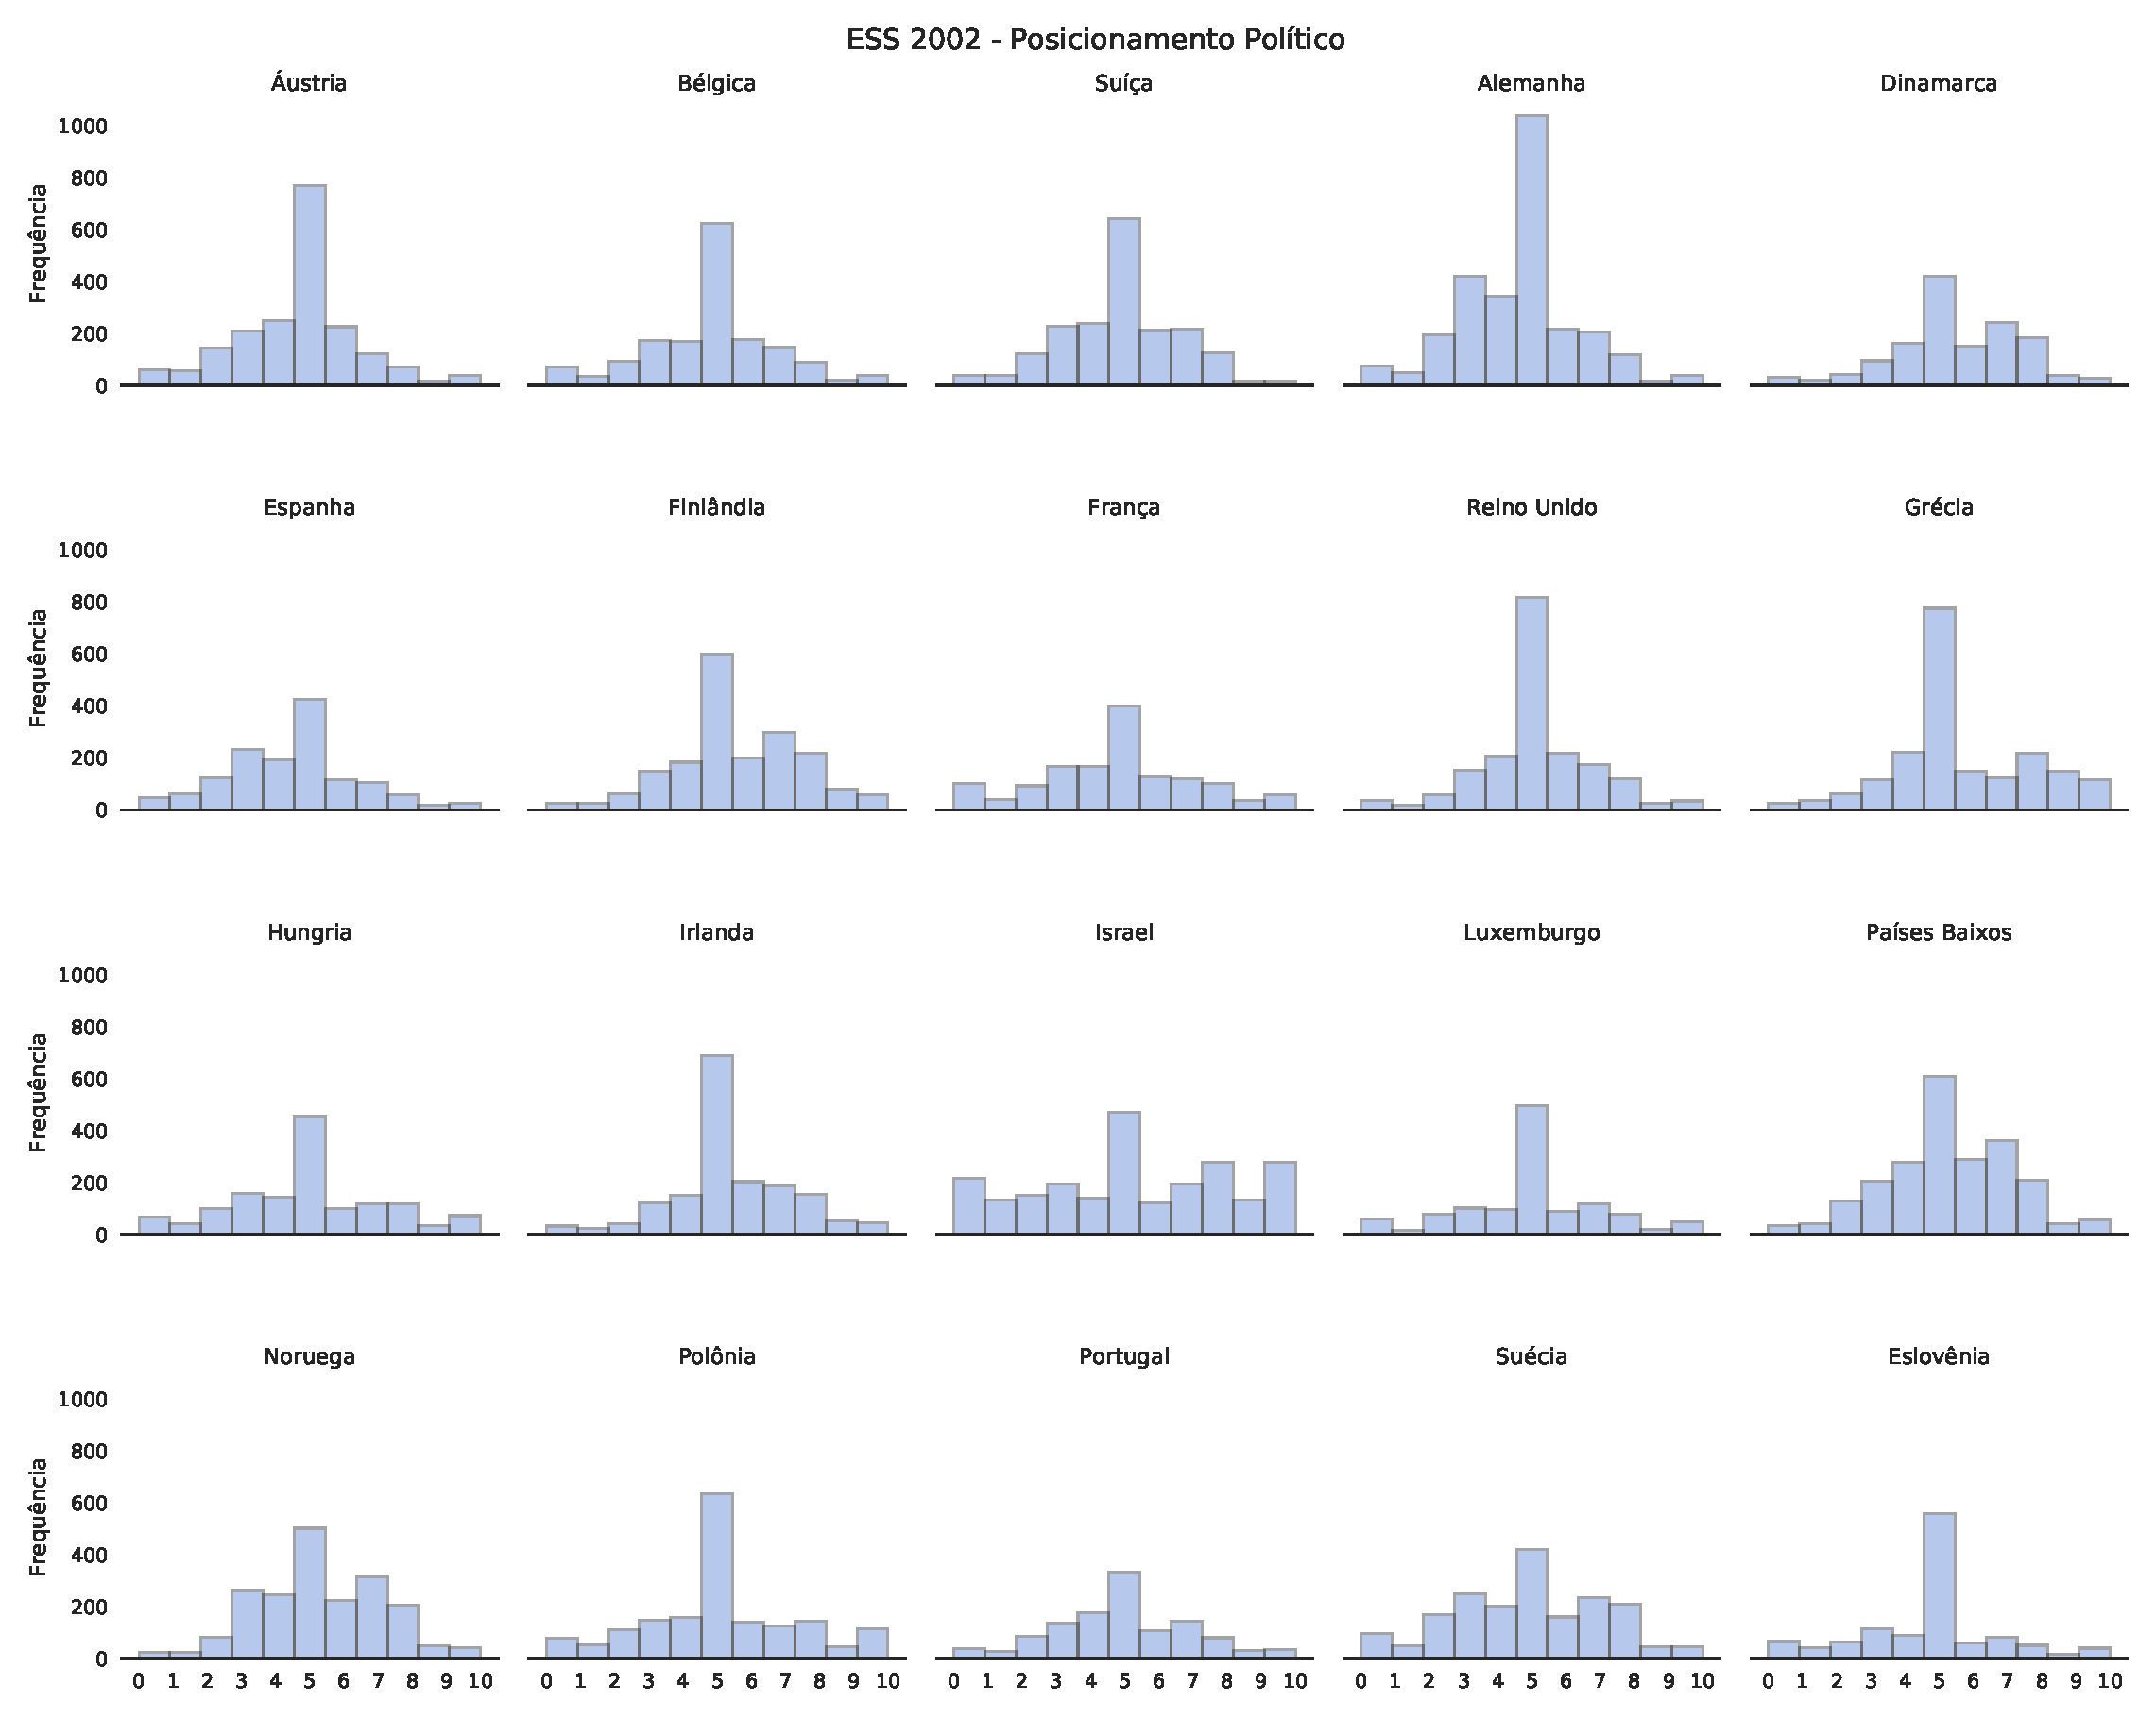
\includegraphics[scale = 0.2]{ims/ess_2002_plots.pdf}
    \caption{ Distribuição de Posicionamento Ideológico de respondentes em 20
      países}
    \label{fig2}
  \end{figure}
\end{frame}


\section{Modelo e Resultados Parciais}


\section*{Referências}
\begin{frame}[allowframebreaks]{Referências}
\printbibliography[heading=none]
\end{frame}

\end{document} 
%%% Local Variables:
%%% mode: latex
%%% TeX-master: ""
%%% End:
